\documentclass[aps,prb,twocolumn,superscriptaddress,nofootinbib,floatfix]{revtex4-1}

\usepackage{amsmath,amssymb,bm}
\usepackage{graphicx}
\usepackage{booktabs}
\usepackage[colorlinks=true,citecolor=blue,linkcolor=blue,urlcolor=blue]{hyperref}

\graphicspath{{../results/}{../figures/}{results/}{figures/}}

\newcommand{\tp}{t'}
\newcommand{\hk}{Hatsugai--Kohmoto}
\newcommand{\mmhk}{MMHK}
\newcommand{\Gs}{G(\mathbf{k},\omega=0)}
\newcommand{\epsk}{\epsilon_{0,\mathbf{k}}}
\newcommand{\els}{\epsilon_{\mathrm{LS}}(\mathbf{k})}

\begin{document}

\title{Capturing 98\% Hubbard Mottness with a Momentum-Mixing Hatsugai--Kohmoto Model}

\author{Peizhi Mai}
\email{peizhimai@gmail.com}
\affiliation{Department of Physics and Institute of Condensed Matter Theory, University of Illinois at Urbana-Champaign, Urbana, Illinois 61801, USA}
\author{Philip W. Phillips}
\email{dimer@illinois.edu}
\affiliation{Department of Physics and Institute of Condensed Matter Theory, University of Illinois at Urbana-Champaign, Urbana, Illinois 61801, USA}
\date{\today}

\begin{abstract}
We use a momentum-mixing Hatsugai--Kohmoto construction as a compact representation of Hubbard Mottness and organize the calculation around four diagnostics: static benchmark observables, doping, next-nearest-neighbor hopping, and the Luttinger surface.  At half filling and $\tp=0$, the $4\times4$ \mmhk{} energy tracks AFQMC and DMET reference data over $U/t=2$--$12$, while the local double occupancy agrees especially well once correlations are appreciable.  For $U/t\ge4$, the double-occupancy deviation from AFQMC is only $0.6$--$2.0\%$; this is the operational sense in which the calculation captures about $98\%$ of the local Mottness benchmark.  The antiferromagnetic moment is less universal, as expected for an order-parameter-like quantity, but follows the same growth toward the Heisenberg-limit scale.  Doping to $n=0.875$ and $n=0.8$ reduces both double occupancy and magnetization, and $\tp=-0.25t$ further suppresses the doped magnetic response while leaving the half-filled curves nearly unchanged.  The momentum-resolved spectra show an interaction-opened gap and a zero of $G(\mathbf{k},0)$ whose dispersion collapses with increasing $U$ onto a scaled noninteracting reference.  The result is a figure-driven benchmark of a minimal model that reproduces the local signatures of Mottness and its associated Green's-function zero surface.
\end{abstract}

\maketitle

\section{Introduction}

The square-lattice Hubbard model is the canonical setting in which itinerant electrons acquire the local constraints, magnetic correlations, and spectral reconstruction associated with Mottness \cite{hubbard1963electron,imada1998metal}.  It is also a stringent benchmark.  Modern numerical methods agree remarkably well on many ground-state energies, but quantities closer to the organizing physics--double occupancy, antiferromagnetic correlations, and momentum-resolved spectra--remain more diagnostic of how a method represents correlations \cite{leblanc2015solutions}.  A useful reduced model should therefore be tested against more than the energy.

The Luttinger surface supplies a complementary momentum-space test.  In a Fermi liquid, the sign of the zero-frequency Green's function changes at a pole.  In a Mott state, the sign change can instead occur through a zero of $G$ \cite{luttinger1960fermi,dzyaloshinskii2003zeros}.  This zero surface records the topology of the low-energy Green's function after quasiparticle spectral weight has been removed.  It is not enough, then, to reproduce local observables and separately draw a zero contour; the two must emerge in the same calculation.

Here we use a momentum-mixing extension of the exactly solvable Hatsugai--Kohmoto construction \cite{hatsugai1992exactly}.  The manuscript is organized directly around the figures.  Figure~\ref{fig:half_filling} asks whether the \mmhk{} model captures the static signatures of Hubbard Mottness.  Figure~\ref{fig:tprime} asks whether those signatures survive doping and next-nearest-neighbor hopping.  Figures~\ref{fig:ls_tp0} and \ref{fig:ls_tpn25} then ask whether the same model produces the expected spectral gap and Luttinger surface for $\tp=0$ and $\tp=-0.25t$.  The answer is affirmative in the local-observable sense: over the correlated regime $U/t\ge4$, the local double occupancy agrees with AFQMC within roughly two percent, while the spectra reveal a robust surface of Green's-function zeros.

\section{Model and diagnostics}

We consider the square-lattice Hubbard Hamiltonian
\begin{equation}
\begin{split}
H ={}&
-t \sum_{\langle ij\rangle,\sigma}
\left(c^\dagger_{i\sigma}c_{j\sigma}+\mathrm{H.c.}\right) \\
&-\tp \sum_{\langle\langle ij\rangle\rangle,\sigma}
\left(c^\dagger_{i\sigma}c_{j\sigma}+\mathrm{H.c.}\right) \\
&+U\sum_i n_{i\uparrow}n_{i\downarrow}
-\mu\sum_{i,\sigma} n_{i\sigma}.
\end{split}
\label{eq:hubbard}
\end{equation}
The benchmark calculations use $4\times4$ clusters and scan total momentum sectors to identify the ground state in each particle-number sector.  For a fixed target density, the chemical potential is determined by solving the grand-canonical density condition; at half filling particle-hole symmetry fixes $\mu=U/2$ for $\tp=0$.  The \mmhk{} construction keeps the interaction local in the momentum-space cluster basis while allowing momentum mixing beyond the purely diagonal Hatsugai--Kohmoto limit.

The observables reported below are the energy per site, the local double occupancy
\begin{equation}
D = \frac{1}{N}\sum_i \langle n_{i\uparrow}n_{i\downarrow}\rangle,
\end{equation}
and the magnetic structure-factor-derived moment used in the benchmark tables.  Momentum-resolved Green's functions are evaluated from particle-addition and particle-removal matrix elements generated in neighboring particle-number sectors.  The zero-frequency Green's function is then used to define the sign field
\begin{equation}
s(\mathbf{k})=\mathrm{sgn}\,\mathrm{Re}\,G(\mathbf{k},0),
\end{equation}
and the Luttinger surface is identified by sign changes of $s(\mathbf{k})$ not associated with a quasiparticle pole.  In the spectral figures we report this zero surface as an effective dispersion $\els$ along the high-symmetry path $\Gamma$--$X$--$M$--$\Gamma$.

\section{Static Mottness Benchmark}

Figure~\ref{fig:half_filling} compares the \mmhk{} results with AFQMC and DMET half-filled benchmarks and also overlays the doped \mmhk{} curves at $n=0.875$ and $n=0.8$.  The energy panel shows that the half-filled \mmhk{} curve follows the reference trend from weak to strong coupling.  It is systematically more negative than the thermodynamic-limit reference values by $0.009$--$0.017t$, corresponding to relative deviations of roughly $1$--$3\%$.  This smooth offset is small on the scale of the Hubbard energy and does not change the interaction dependence.

The double-occupancy panel is the central local-Mottness benchmark.  At $U/t=2$, the \mmhk{} value $D=0.1850$ is below the AFQMC value $0.1923(3)$, reflecting a modest overestimate of correlation effects in the weak-to-intermediate crossover.  For $U/t\ge4$, however, the absolute deviation from AFQMC is only $5.7\times10^{-4}$--$1.1\times10^{-3}$, or $0.6$--$2.0\%$.  Thus the model captures at least about $98\%$ of the benchmark local Mottness over the correlated regime.  Doping reduces $D$ at fixed $U$, as expected when the local Mott constraint is weakened by holes.

The magnetization panel behaves differently.  The \mmhk{} moment grows from $m=0.174$ at $U/t=2$ to $m=0.292$ at $U/t=12$ and approaches the two-dimensional Heisenberg-limit scale indicated in the figure, but its agreement with AFQMC and DMET is not as uniform as that of $D$.  This is the expected hierarchy: local charge observables are more robust, while magnetic order parameters are sensitive to finite-size geometry, symmetry constraints, and the extraction of long-distance spin correlations.

\begin{figure*}[p]
  \centering
  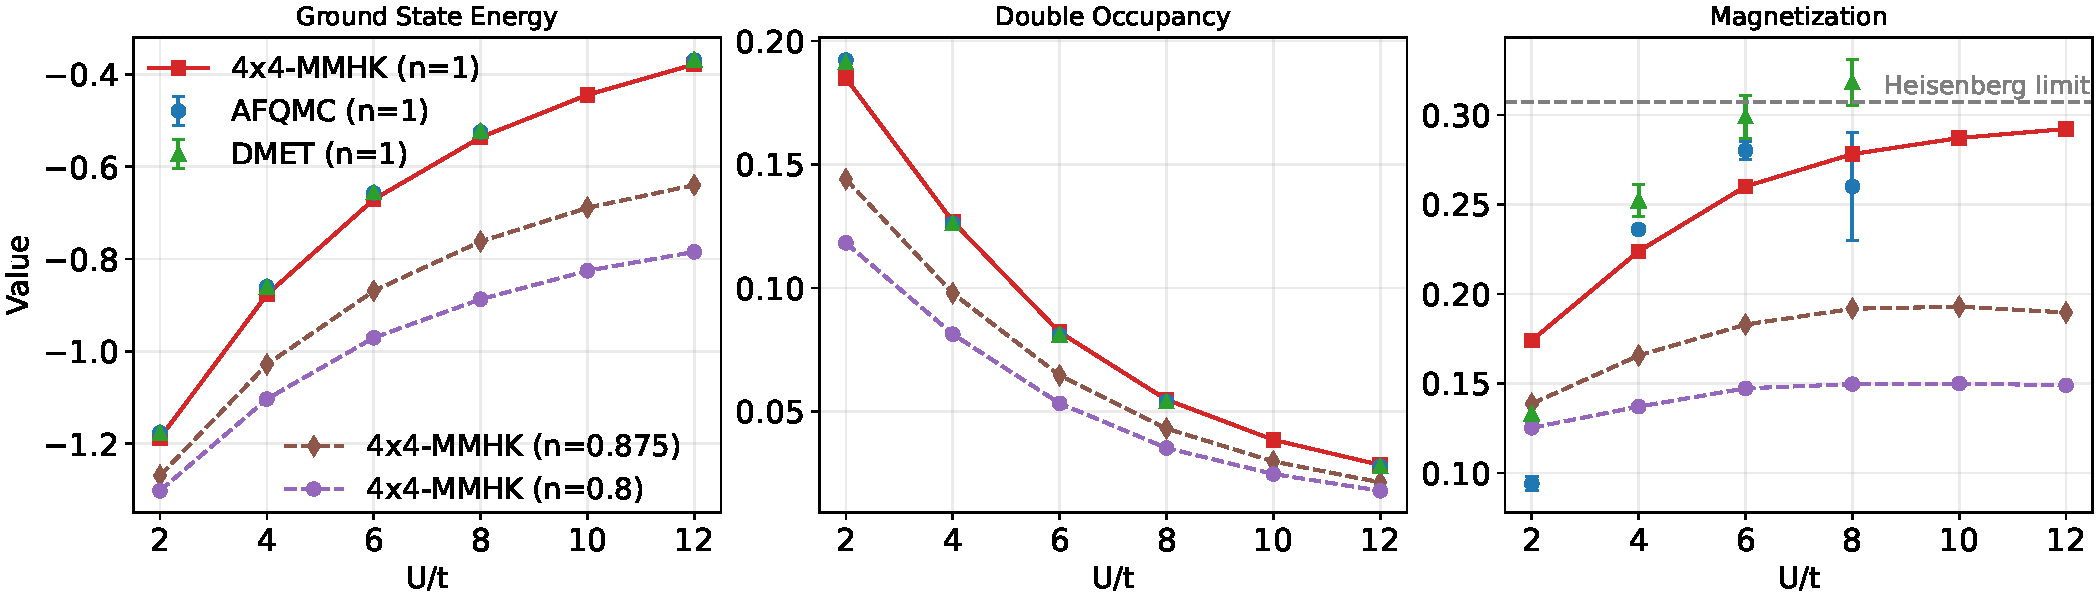
\includegraphics[width=\textwidth]{half_filling_comparison.pdf}
  \caption{
  Static benchmark and doping trends at $\tp=0$.  Ground-state energy, double occupancy, and magnetic moment are shown as functions of $U/t$.  The half-filled \mmhk{} data are compared with AFQMC and DMET benchmarks from Ref.~\onlinecite{leblanc2015solutions}; doped \mmhk{} results at $n=0.875$ and $n=0.8$ are included to show how the same observables evolve away from half filling.  The local double occupancy is the sharpest benchmark: for $U/t\ge4$, \mmhk{} differs from AFQMC by about $0.6$--$2.0$ percent.
  }
  \label{fig:half_filling}
\end{figure*}

\section{Doping and Next-Nearest-Neighbor Hopping}

Figure~\ref{fig:tprime} isolates the effect of $\tp=-0.25t$ over the range $U/t=6$--$12$.  At half filling, the solid and dashed red curves nearly coincide in all three panels.  This is consistent with the fact that, for the finite cluster and observables considered here, the local half-filled response is dominated by $U$ rather than by the modest next-nearest-neighbor hopping.

Away from half filling, $\tp$ matters more.  At $n=0.875$, the magnetization is reduced from $m=0.190$ to $m=0.175$ at $U/t=12$ when $\tp=-0.25t$ is introduced.  At $n=0.8$, the same comparison gives a reduction from $m=0.149$ to $m=0.134$.  The local double occupancy is also lower with $\tp=-0.25t$: at $n=0.8$ and $U/t=12$, it decreases from $0.0179$ to $0.0135$.  The figure therefore separates two effects that are often conflated: doping weakens the Mott and magnetic response, while next-nearest-neighbor hopping further frustrates the doped magnetic correlations.

\begin{figure*}[p]
  \centering
  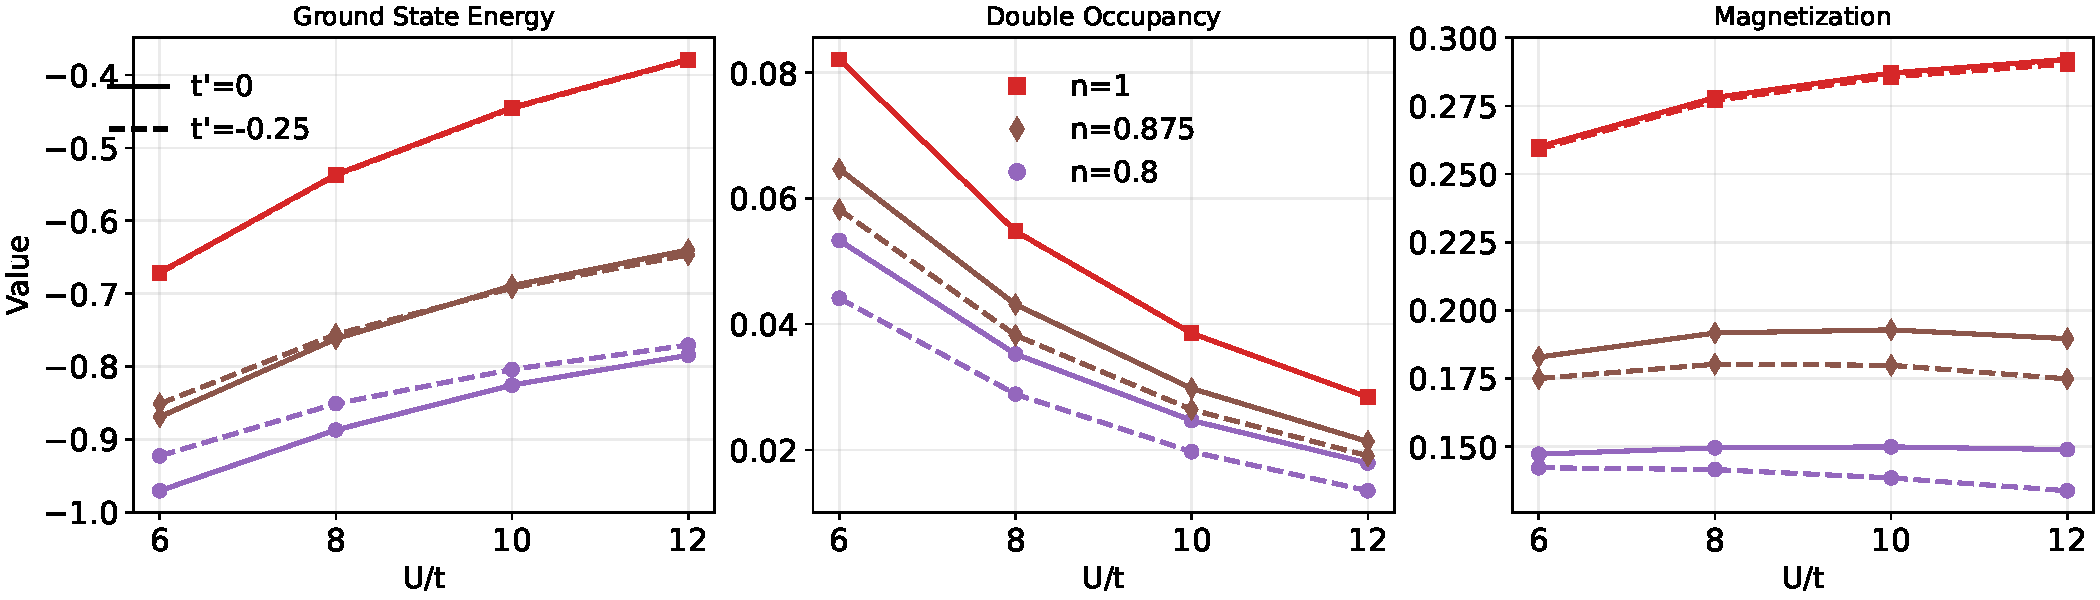
\includegraphics[width=\textwidth]{tprime_overlay_comparison.pdf}
  \caption{
  Effect of next-nearest-neighbor hopping.  Solid curves show $\tp=0$ and dashed curves show $\tp=-0.25t$ for $n=1$, $0.875$, and $0.8$.  The half-filled curves are nearly unchanged by $\tp$, while the doped double occupancy and magnetization are reduced by finite $\tp$.  The suppression is most visible in the magnetic panel, where $\tp=-0.25t$ lowers the $n=0.8$ moment from about $0.149$ to $0.134$ at $U/t=12$.
  }
  \label{fig:tprime}
\end{figure*}

\clearpage

\section{Spectra and Luttinger Surface}

Having established the static benchmark, we turn to the momentum-resolved spectra in Figs.~\ref{fig:ls_tp0} and \ref{fig:ls_tpn25}.  The color maps show spectral weight along $\Gamma$--$X$--$M$--$\Gamma$ for $U/t=8$, $12$, $20$, and $40$.  In all cases the spectral weight is expelled from $\omega=0$, producing a Mott gap.  The white curve marks the extracted zero of $G(\mathbf{k},0)$, or equivalently the Luttinger-surface dispersion $\els$ along the same path.

The important feature is the separation between poles and zeros.  The red spectral-weight ridges are pushed to Hubbard-band energies that scale with $U$, while the white zero contour remains near the low-energy band geometry and crosses the high-symmetry path where the sign of $G(\mathbf{k},0)$ changes.  Thus the momentum-space sign structure survives even though no quasiparticle pole remains at the chemical potential.

For $\tp=0$, Fig.~\ref{fig:ls_tp0}(e) shows that the extracted $\els$ curves for $U/t=8$, $12$, $20$, and $40$ collapse onto a common shape.  Panel (f) compares the $U/t=40$ curve with the plotted scaled noninteracting dispersion, $-1.4\epsk$, and the agreement is nearly pointwise.  In this sense the strong-coupling Luttinger surface retains the geometry of the underlying band even after the spectral poles have moved to Hubbard-band energies.

\begin{figure*}[p]
  \centering
  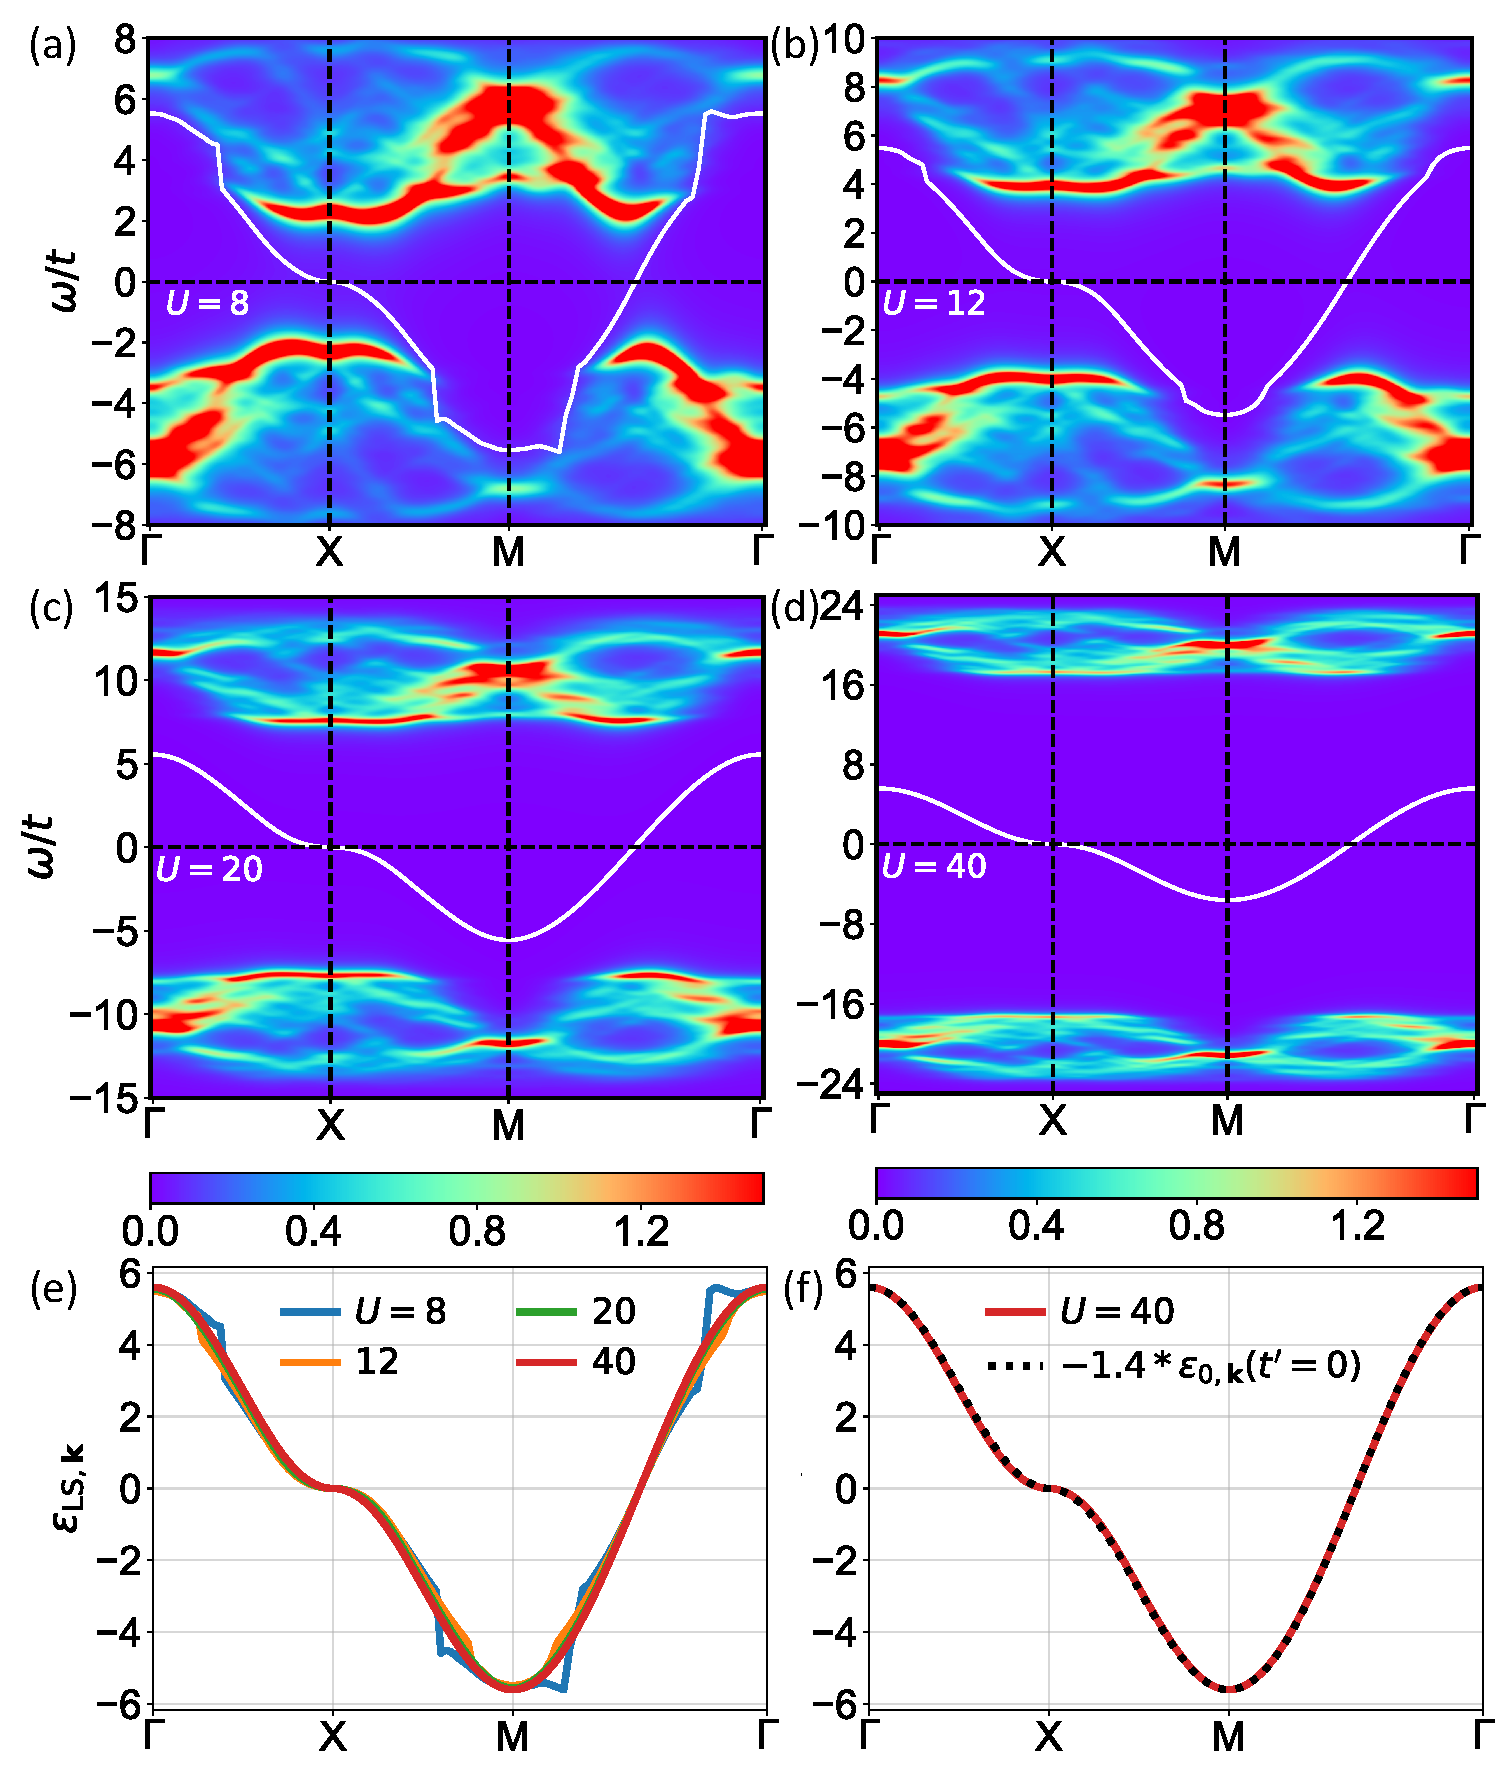
\includegraphics[width=0.72\textwidth]{hftp0.pdf}
  \caption{
  Spectral function and Luttinger surface for $\tp=0$.  Panels (a)--(d) show the spectral function along $\Gamma$--$X$--$M$--$\Gamma$ for $U/t=8$, $12$, $20$, and $40$; the white curve is the extracted zero of $G(\mathbf{k},0)$.  Panel (e) overlays the corresponding Luttinger-surface dispersions, showing their collapse with increasing $U$.  Panel (f) compares the $U/t=40$ Luttinger-surface dispersion with the plotted scaled noninteracting reference, $-1.4\epsk$.
  }
  \label{fig:ls_tp0}
\end{figure*}

The same structure persists for $\tp=-0.25t$, shown in Fig.~\ref{fig:ls_tpn25}.  The finite $\tp$ shifts the underlying dispersion and therefore shifts the zero contour, most visibly near the $X$--$M$ portion of the path.  Nevertheless, the qualitative behavior is unchanged: the spectral gap grows with $U$, the zero contour remains sharply defined, and the large-$U$ Luttinger-surface dispersion is again well described by a scaled noninteracting reference.  This robustness is the momentum-space counterpart of the static result in Fig.~\ref{fig:tprime}: finite $\tp$ modifies details, especially away from half filling, but does not destroy the Mottness encoded by the Green's-function zero.

\begin{figure*}[p]
  \centering
  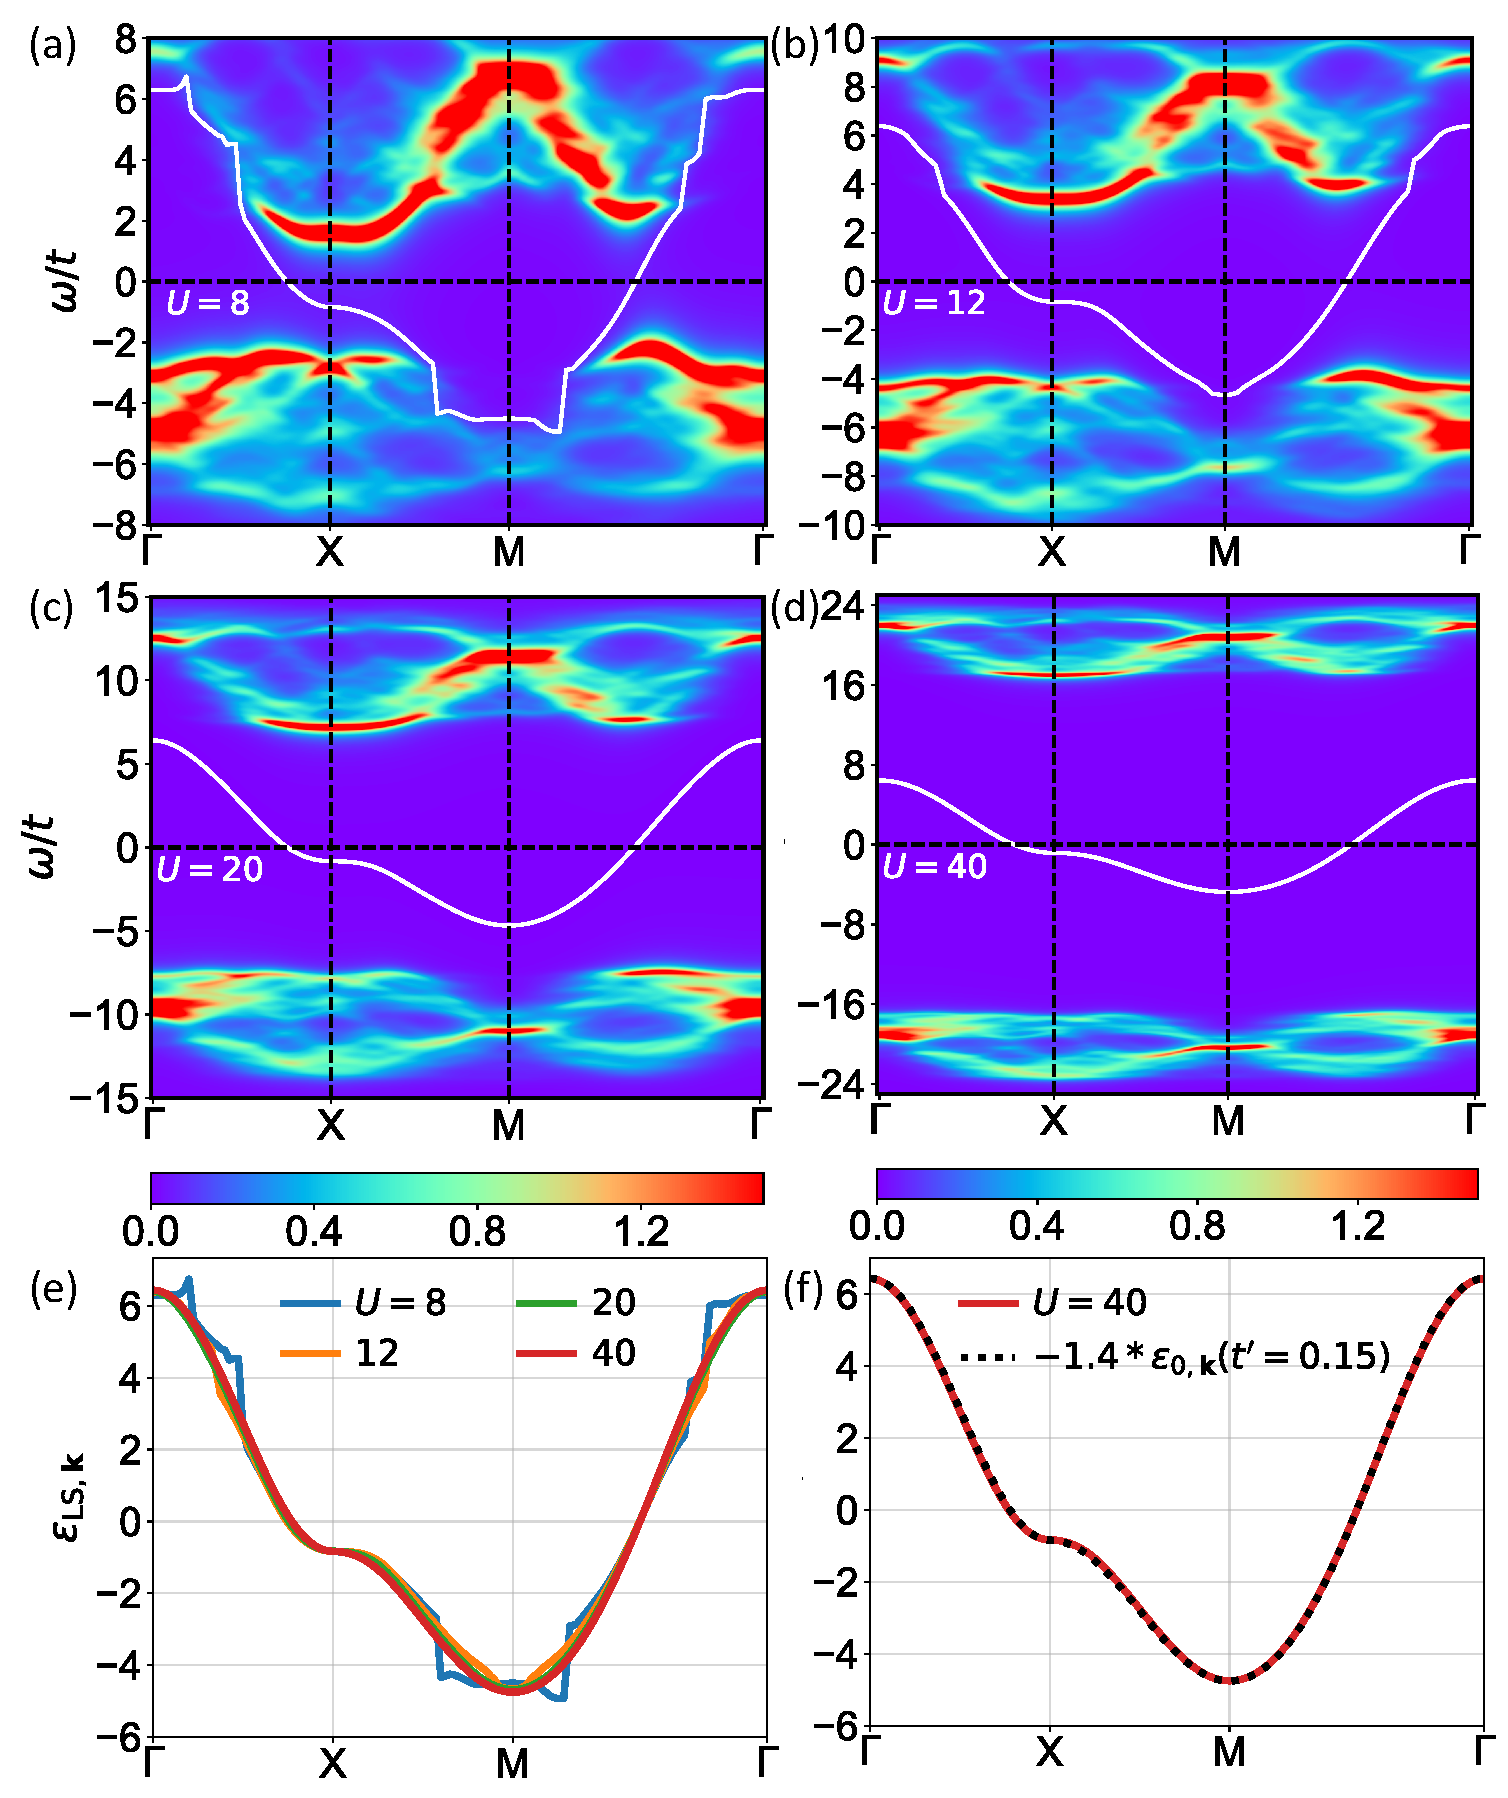
\includegraphics[width=0.72\textwidth]{hftpn25.pdf}
  \caption{
  Spectral function and Luttinger surface for $\tp=-0.25t$.  Panels (a)--(d) show the interaction evolution of the spectrum and the zero of $G(\mathbf{k},0)$.  Panel (e) shows that the extracted Luttinger-surface dispersions remain close to one another as $U$ increases.  Panel (f) compares the strong-coupling dispersion with the corresponding scaled noninteracting reference.  Finite $\tp$ shifts the zero contour but preserves the pole-zero separation characteristic of a Mott state.
  }
  \label{fig:ls_tpn25}
\end{figure*}

\clearpage

\section{Discussion}

The figures establish a hierarchy of confidence.  The strongest quantitative agreement is in the local double occupancy, which is the most direct static measure of Mottness in this calculation.  The ground-state energy has a small smooth offset, but follows the correct interaction dependence.  The magnetization is the least universal of the three static quantities, as already seen in method comparisons of the Hubbard model \cite{leblanc2015solutions}.  This is why the title's $98\%$ claim should be read as a local-Mottness statement rather than as a claim that every observable agrees at the two-percent level.

The spectral figures add a second, independent check.  A model could reproduce $D$ while giving the wrong momentum-space sign structure.  Here the same \mmhk{} calculation produces both the local suppression of double occupancy and a zero surface of $G(\mathbf{k},0)$.  The collapse of $\els$ with increasing $U$, and its close agreement with a scaled noninteracting dispersion at $U/t=40$, suggest that the strong-coupling zero surface is controlled primarily by the underlying band geometry, while the poles are expelled to high energies.  This is precisely the pole-zero separation expected of a Mott state.

\section{Conclusion}

We have reorganized the \mmhk{} benchmark around the information contained in the figures.  The static data show that the model captures the interaction dependence of the Hubbard energy, double occupancy, and magnetization, with the cleanest quantitative agreement in the local double occupancy.  For $U/t\ge4$, the double occupancy agrees with AFQMC to within about two percent, motivating the statement that the model captures roughly $98\%$ of the local Hubbard Mottness.  Doping and $\tp=-0.25t$ reduce the local and magnetic responses in the expected way.  The spectral data then show that this same calculation produces a robust Luttinger surface: the zero of $G(\mathbf{k},0)$ survives after the low-energy spectral poles are removed and, at strong coupling, follows a scaled noninteracting dispersion.  The \mmhk{} construction therefore provides a compact route from benchmarked local Mottness to the Green's-function zero structure of the Mott state.

\begin{acknowledgments}
We thank [names] for useful discussions.  This work used computational resources at [facility].
\end{acknowledgments}

\bibliographystyle{apsrev4-1}
\IfFileExists{references.bib}{\bibliography{references}}{\bibliography{manuscript/references}}

\end{document}
